\documentclass[9pt,journal,compsoc]{IEEEtran}
\usepackage[utf8x]{inputenc}
\usepackage{xcolor}
\usepackage{listings}
\usepackage{cite}
\usepackage{caption}
\usepackage{graphicx}
\usepackage{sectsty}
\usepackage{blindtext}
\usepackage{newcent}
\usepackage[T1]{fontenc}
\usepackage{tgbonum}
\usepackage{amsmath}
\usepackage{etoolbox}

\makeatletter

\pagecolor{white}
\renewcommand {\thesectiondis} {\Roman{section}}
\renewcommand {\thesubsectiondis} {\thesectiondis.\Alph{subsection}}
\renewcommand {\thesubsubsectiondis}{\thesubsectiondis.\arabic{subsubsection}}


\title{Qantum walks}
\author{Dauliac, Julien}
\date{December 2022}

\begin{document}

    \maketitle
    
    \section{Introduction}
        Markov chains are a mathematical tool describing probabilistic dynamic systems \cite{motwani1995randomized}.
        They play an important role in randomized algorithms (e.g., continuous approximation algorithms and other difficult problems, and volume estimation)
        Random walks are an example of Markov processes, in which future behaviour is independent of past history
        
        Quantum walks are their equivalents in the quantum world. They share many properties but are also remarkable for some particularities.        
        \begin{figure}[htp!]
            \centering
            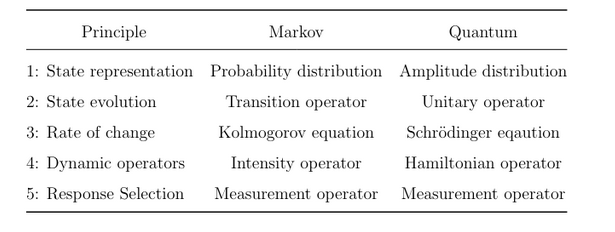
\includegraphics[scale=0.34]{assets/img/forked-graph.png}
            \caption{Comparative table of the main dynamics underlying markov chains walkers and quantum walkers models. Fig 1 from \cite{busemeyer2020comparison}}
            \label{fig:diff}
        \end{figure}

        The walkers in the markov chains move according to a random distribution of one node at a time in each iteration. They ultimately occupy a unique place at each time.
        The unobserved quantum walkers, not being in a defined state, move following an amplitude probability or "simultaneously" according to their statistical distribution to all possible next nodes:
        \begin{figure}[htp!]
            \centering
            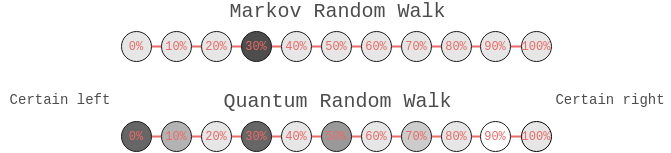
\includegraphics[width=\linewidth]{assets/img/schema3.png}
            \caption{Illustration opposing the two walk systems. Inspired by Figure 2 from \cite{busemeyer2020comparison}}
            \label{fig:opposing}
        \end{figure}
        
        
    \section{Applications}
        Quantum walks have many applications. They are both inherited from markov chains but also have new uses.
        
        \subsection{Continuous walks}
            Quantum walkers are able to describe discrete displacements like their classical counterparts. However, they are also able to easily describe continuous walks, and this by exploiting their intrinsics physical properties \cite{kendon2020compute}.
            Let's assume superposed quantum walkers:
            $$ \alpha \lvert \text{0}\rangle + \beta \lvert\text{1}\rangle$$
            Qbits can change smoothly from a probability of $0$ to $1$ or anything in between. Their value is naturally statistical and therefore continuous and suitable for this purpose.

        \subsection{Algorithmes}

        \subsubsection{Search}
            Search is one of the big families of problems in computer science and markov chains offer a framework to address them.
            
            Quantum walks are also capable of addressing them, but they offer higher quadratic complexity than classical algorithms \cite{santha2008quantum}.
        
        \paragraph{Groover search algorithm}
            The algorithms for searching in unordered graphs are very efficient.
            For example We can look at a walk variant of the Groover search algorithm \cite{ santha2008quantum}.
            We consider two search algorithms based on some ergodic and symmetric chain.
            For a number of node $n$, in the normal world, the search cost is
            $$ cost_c = O(\frac{1}{n}) $$.
            In the quantum world, if we consider the setup and verification cost at $ S+C = O(1)$.
            Then we can set search cost to be
            $$ cost_q =  \frac{1}{\sqrt{n}}$$
            We can observe the quadratic difference in cost from one algorithm to another
            $$ cost_q < cost_n$$
            
        \subsubsection{Simulations}
            Another interesting use of quantum walks is the simulation of physical elements.
                
            For example, we could simulate economic models \cite{orrell2021quantum}
            or physical particles, like neutrinos \cite{di2016quantum} or photons \cite{aspuru2012photonic}.

            Chemical simulations could also be performed thank's to quantum walks \cite{kassal2011simulating}.
            Since these simulations have a high computational complexity due to the number of combinations to be tested, quantum systems could help to reduce this complexity in order to make these calculations affordable.

            It is also possible using the QFold algorithm to combine quantum computing with deep learning methods to predict the 3D structure of proteins  \cite{casares2022qfold}

    
    \section{Detail and comparison of a discrete walk}
        In this part we will take the example of the random exploration of a graph to highlight the properties of quantum walks.
        The quantum walk processes are not so different from those concerning walks on Markov chains. As we will see the biggest difference is in the observed results
        
        \subsection{Setup}
            The studied graph will be cyclic. It has 8 nodes and the probabilities of joining one node or another will be equivalent.
            $$p = \frac{1}{2}$$.
            It is possible to represent the walker on $n$ bits or qbit.
            In our example, we will use 6 bits to represent the 64 nodes: $2^6=64$.
            \begin{figure}[htp!]
                \centering
                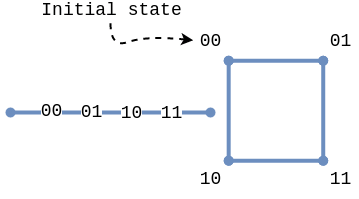
\includegraphics[scale=0.4]{assets/img/schema1-bis.png}
                \caption{Here is an example representing a quantum walker on a graph of 4 nodes encoded in 2 bits}
                \label{fig:encoding}
            \end{figure}
            
            We will use 2 logic gates incrementing and decrementing our bit in order to choose if we go forward or backward. This is our unitary operator.
            \begin{figure}[htp!]
                \centering
                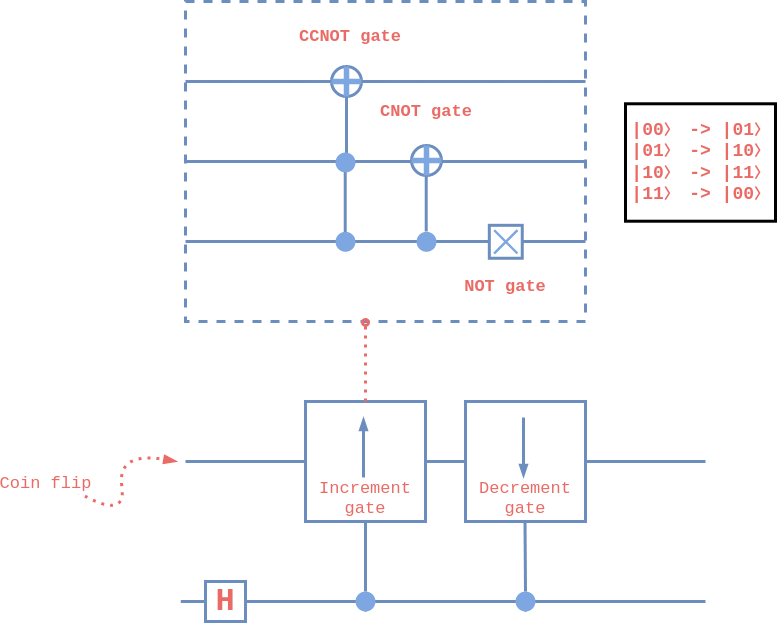
\includegraphics[width=\linewidth]{assets/img/schema2.png}
                \caption{Here is an example representing a quantum walker on a graph of 4 nodes encoded in 2 bits}
                \label{fig:opposing}
            \end{figure}
            
            We will use a coin to decide which direction to take on our graph. This coin being a random draw in the normal world.
            In the quantum world we will use the most used gate for the quantum walk pieces: Hadamard's gate.
            \begin{equation*}
            \begin{split}
                H & = \frac{1}{\sqrt{2}}\begin{pmatrix} 1 && 1 \\ 1 && -1 \end{pmatrix} \Rightarrow  H \lvert  \uparrow\rangle
                \\
                &= \frac{\lvert\uparrow\rangle  + \lvert  \downarrow\rangle }{\sqrt{2}} \ \Rightarrow \ H \lvert  \downarrow\rangle
                \\
                &= \ \frac{\lvert  \uparrow\rangle  - \lvert  \downarrow\rangle }{\sqrt{2}}
            \end{split}
            \end{equation*}

    \section{Runtime}
        If the initial state of our part before throwing is \lvert n,\uparrow\rangle$.
        
        It will be after throwing of 
        $$\frac{1}{\sqrt{2}} \lvert n, \uparrow\rangle+ \frac{1}{\sqrt{2}} \lvert n, \downarrow\rangle $$

        The result of the first two steps is quite similar.
        If, after the second step, we measure a state $n = -2$ (heads on the previous move) and $n = 2$ (tails on the previous move) with probability $\frac{1}{4}$ and $n = 0$ with probability $\frac{1}{2}$.
        This is exactly what we would have obtained in a classic march.
        The third step is different. In the coin flip step, the state:
        $$\frac{1}{2} \lvert 0, \downarrow\rangle + \frac{1}{2} \lvert 0, \uparrow\rangle$$
        is transformed into \cite{ambainis2003quantum}:
        $$\frac{1}{\sqrt{2}} \lvert 0, \uparrow\rangle$$ 
        
        In a classical random walk, we choose the left and right direction with probabilities $\frac{1}{2}$ each.
        In the quantum case, because of the quantum interference and the initial state of the coin qbit, we choose to go left with the full probability amplitude \cite{Knight2003QuantumWO} \label{interfereces}.

        \begin{figure}[htp!]
            \centering
            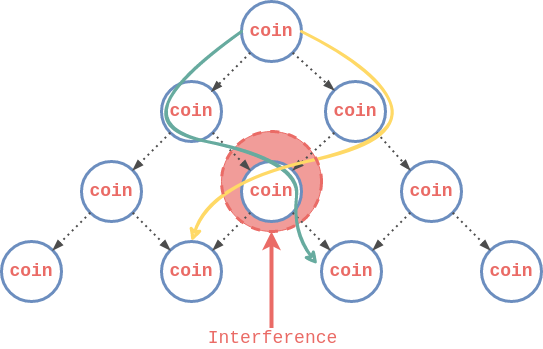
\includegraphics[width=\linewidth]{assets/img/schema4.png}
            \caption{Illustration of interference cases in the context of quantum walks. Inspired by \cite{AuantumEconomicsAndFinance2021}}
            \label{fig:opposing}
        \end{figure}
        If we simulate a classical random walker, we will obtain a normal distribution of the type:
        \begin{figure}[htp!]
            \centering
            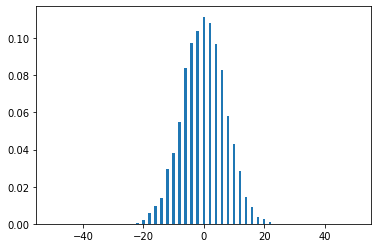
\includegraphics[scale=0.4]{assets/img/normal.png}
            \caption{Normal distrubution \cite{QuantumDemoDauliac2022}}
            \label{fig:opposing}
        \end{figure}
        We use 7 qbits instead of 3 to have better graphic représentation.

        In the case of our quantum walker we will get the following distribution.
        It is important to note that the graphs will only have even or odd data points, depending on the initial position of the walker. and the number of steps taken.
        \begin{figure}[htp!]
            \centering
            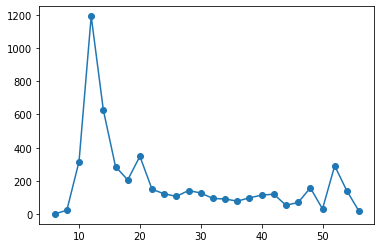
\includegraphics[scale=0.4]{assets/img/quantum_left_distribution.png}
            \caption{Quantum biased distrubution \cite{QuantumDemoDauliac2022}}
            \label{fig:opposing}
        \end{figure}

        The central collapse being due to the quantum interferences evoked in the unwinding part \ref{interfereces}
        We will obtain the inverse state if our qbit is initialized in the $\lvert\uparrow\rangle$ to note that the graphs will only have even or odd data points, depending on the initial position of the walker. and the number of steps taken. The central collapse being due to the quantum interferences evoked in the part 4. We will obtain the inverse state if our qbit is initialized in$\lvert\downarrow\rangle$ state.

        \begin{figure}[htp!]
            \centering
            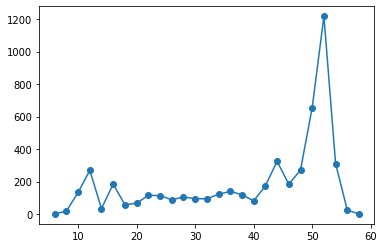
\includegraphics[scale=0.4]{assets/img/quantum_right_distribution.png}
            \caption{Quantum biased distrubution 2\cite{QuantumDemoDauliac2022}}
            \label{fig:opposing}
        \end{figure}
        
        If we initialize our corner qbit to a "balanced" state, interference should not bias our distribution:
        $$\lvert i\rangle \ = \ \frac{\lvert\uparrow\rangle \ + \ i\lvert\downarrow\rangle}{\sqrt{2}}$$

        We proceed by applying a hadamar gate $S$ then a phase gate $S$ on our qbit \cite{morvan2021qutrit}.
        
        We will therefore obtain the following unbiased result \cite{kempe2003quantum} \cite{quantumaiQuantumWalk}:
        \begin{figure}[htp!]
            \centering
            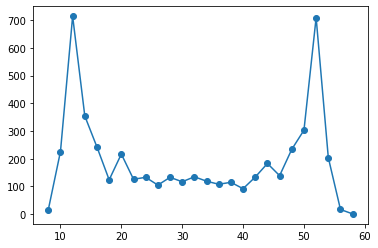
\includegraphics[scale=0.4]{assets/img/quantum_distribution.png}
            \caption{Quantum distrubution\cite{QuantumDemoDauliac2022}}
            \label{fig:opposing}
        \end{figure}
        In the case of a classical random walk, we can observe $\sigma^2 \sim \ T$ where $\sigma$ is the standard deviation and $\T$ is the number of time steps.
        In the case of a quantum walk $\sigma^2 \sim \ T^2$.
        This means that the standard deviation in the case of a quantum walker grows quadratically faster.
        The quantum walker explores, spreads quadratically faster than the classical one.


    \section{Conclusion}
    
        In conclusion, quantum walks are a computing tool with extremely powerful exploitable physical characteristics.
        It is theoretically possible to put them to work on a number of problems, whether to optimize existing algorithms, or to discover new ones opening new perspectives.
    \nocite{*}
    
    \bibliographystyle{IEEEtran}
    \bibliography{references}
    
\end{document}
